\section{Workload Metrics}
We are now in a position to combine the three categories of workload (cognitive, algorithmic, and temporal) with the formal model of the actors and team to generate a set of workload metrics.  Because the categories include many possible measurements that are beyond the scope of this paper, we use labels for the workload metrics that are slightly different from the workload categories.  As shown in Figure~\ref{fig:WorkloadMetrics}, cognitive workload or resource workload as it is termed in this work, is measured using metrics under the {\em resource} workload label, algorithmic under {\em decision}, and temporal workload is labeled the same. 


\begin{figure}[h]
\center
\setlength{\abovecaptionskip}{1mm}
\setlength{\belowcaptionskip}{1mm}
\setlength{\textfloatsep}{1mm}
\setlength{\floatsep}{1mm}
\scalebox{.8}{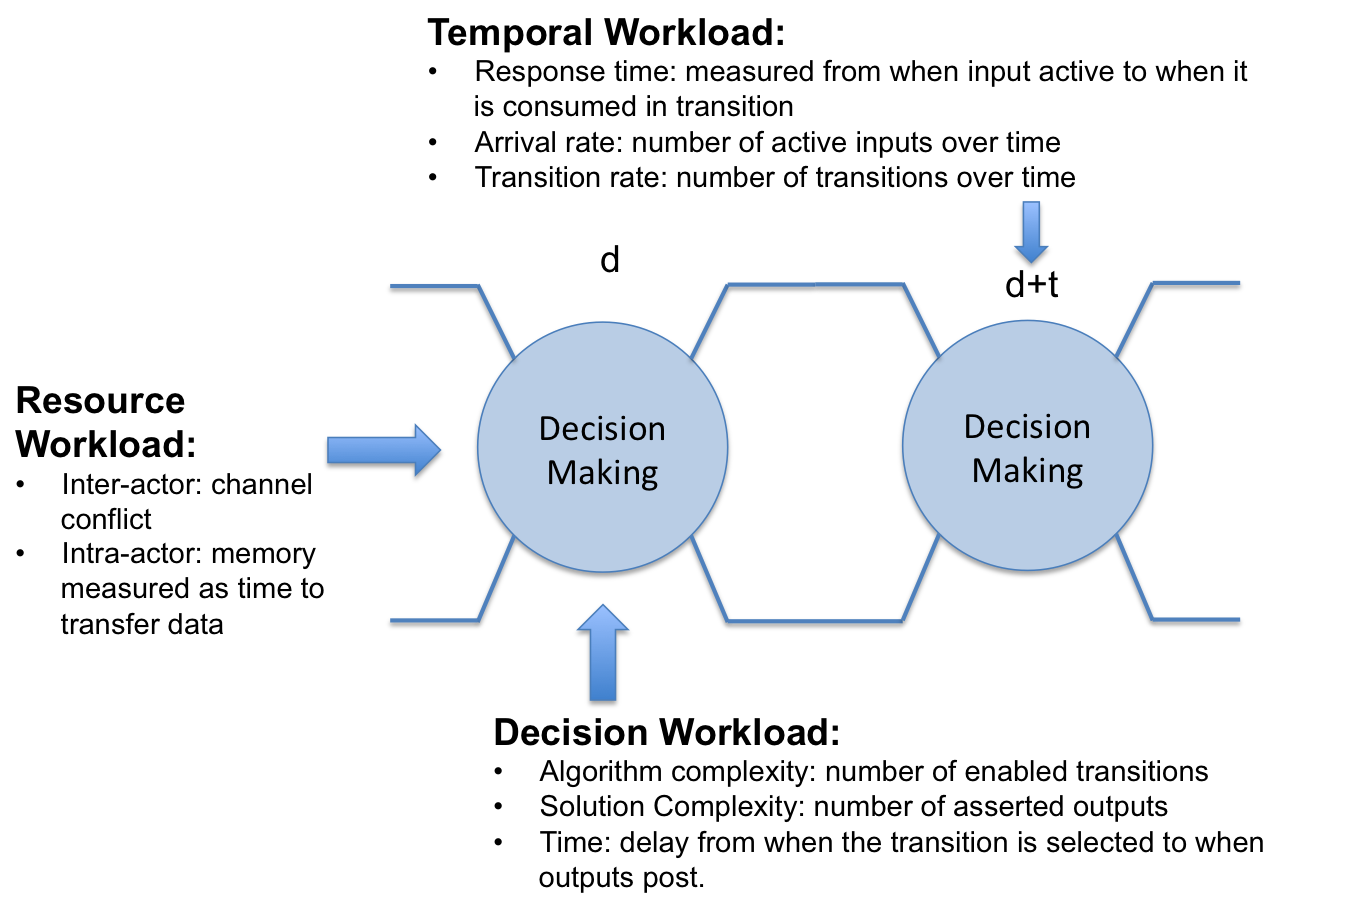
\includegraphics[height=2.5in]{WorkloadMetrics.png}}
\caption{Workload in the model.}
\label{fig:WorkloadMetrics}
\end{figure}

Resource workload is separated into both inter-actor communication and actor
memory load. Decision workload can be broken down into timing, algorithm complexity, and complexity of the solution. Temporal workload includes operations tempo, arrival rate, and response time.

Java Pathfinder (JPF) is a tool used to explore all points of nondeterminism.
%find all possible paths represented in Java source code. 
It does this by compiling the source code as a JPF binary and
running it in a virtual machine. The virtual machine can dynamically alter
sections of the program and concurrently generate and run copies of the program
based off of these changes. This allows us to include alterable values in our
model and simulate an array of different actors without the need to modify the
model.

We have set up a JPF listener to record workload. A JPF listener is a tool that
follows the Listener Design Pattern and acts in the expected fashion. We have
focused our listeners on three pieces of the model: the active inputs, enabled
transitions, and the time taken to perform a transition. We then use these
pieces of the model to represent resource, decision, and temporal workload respectively.
